\documentclass[a4paper, 14pt]{extarticle}

\usepackage{amsmath}
\usepackage{amssymb}
\usepackage{amsthm}
\usepackage{commath}
\usepackage[margin=0.5in]{geometry}
% \usepackage{lexend}
\usepackage{microtype}
\usepackage{parskip}
\usepackage{tikz}
\usepackage{tikz-cd}
\usepackage{tkz-euclide}
\usepackage{xparse}

\usetikzlibrary{calc,angles,quotes, positioning, shapes.geometric}

\theoremstyle{definition}
\newtheorem{dfn}{Definition}
\newtheorem{clm}{Claim}
\newtheorem{asn}{Assertion}
\newtheorem{thm}{Theorem}
\newtheorem{prb}{Problem}
\newtheorem{ans}{Answer}
\newtheorem{lm}{Lemma}
\newtheorem{rmk}{Remark}
\newtheorem{crl}{Corollary}
\newtheorem{ex}{Exercise}
\newtheorem{xmp}{Example}

\newcommand{\titleheader}[1]{\begin{centering}
\begin{LARGE}
\textbf{#1}
\end{LARGE}\\
\hrulefill

\vspace{-1.25\baselineskip}
\hrulefill
\end{centering}\\\\}

\def\changemargin#1#2{\list{}{\rightmargin#2\leftmargin#1}\item[]}
\let\endchangemargin=\endlist

\NewDocumentEnvironment{smrg}{}{\begin{changemargin}{0.5cm}{0.5cm}}{\end{changemargin}}

\NewDocumentEnvironment{SWP}{m m}
{%
  \vspace{-.9cm}%
  \begin{changemargin}{0.5cm}{0.5cm}%
  \noindent#1~#2
  \par
  \textbf{Proof.} 
}
{%
  \qed
  \end{changemargin}
}

\NewDocumentEnvironment{SNP}{m}
{%
  \vspace{-.9cm}%
  \begin{changemargin}{0.5cm}{0.5cm}%
  \noindent#1
}
{%
  \end{changemargin}
}

\newcommand{\bb}[1]{\mathbb{#1}}
\newcommand{\st}{\space \mid \space}
\newcommand{\union}[1]{\displaystyle\mathop{\cup}\limits_{#1}}
\newcommand{\intersect}[1]{\displaystyle\mathop{\cap}\limits_{#1}}
\newcommand{\paran}[1]{\left ( {#1} \right )}
\newcommand{\contra}{$\rightarrow\!\leftarrow$}
\newcommand{\kvec}[2]{({#1}_1 \dots {#1}_{#2})}
\newcommand{\pf}{\textbf{Proof.} }

\newcommand{\AnswerSection}{
    \newpage
    \section*{Answers to Exercises}
    \textit{The following are brief solutions or hints. You are encouraged to review the exercises before checking the answers.}
}
\begin{document}
\titleheader{Properties of $\bb R$}
\textbf{Prereqs} RA-04, FD-01

We now look at two properties of  $\bb R$.
\begin{SNP}{\thm}{$\bb{N}$ is unbounded in $\bb{R}$}
\end{SNP}
That is, if we regard $\bb N$ as a subset of $\bb R$, it is not bounded. i.e, there is no fixed number $x$ such that every natural number is smaller than $x$. I realise this might seem obvious, but try proving this for $\bb Q$, and you'll see it's not that trivial.
\begin{smrg}
\pf Suppose, for contradiction, that $\bb N$ is bounded in $\bb R$. Certainly, $1 \in \bb N$ therefore $\bb N$ is also nonempty. Thus, by completeness, $\bb N$ has a least upper bound, say $\alpha$.

Since $\alpha$ is an upper bound of $\bb N$, it follows that 
$$n \leq \alpha$$for every $n$. However, $n + 1$ is a natural number for every $n$. Thus it follows that
\begin{align*}
n + 1 \leq \alpha\\
\iff n \leq \alpha - 1
\end{align*}
for every $n$. This entails $\alpha - 1$ is an upper bound of $\bb N$. But $\alpha$ was supposed to be the least upper bound on $\bb N$\contra

$\bb N$ cannot admit an upper bound.\qed
\end{smrg}

This is called the \emph{Archimedean Property} of $\bb R$. In literature, often this is referred to as \emph{version 1} of the property. We'll now state and prove version 2.

\begin{SWP}{\thm}{For every $x, y \in \bb R$ such that $x > 0$, there is some $n \in \bb N$ such that $nx \geq y$}
If $y \leq 0$ then $n = 1$ satisfies the property, so suppose $y > 0$. We know from version 1 that $\bb N$ has no upper bound. Therefore, in particular, $\frac{y}{x}$ is not an upper bound of $\bb N$, i.e there exists some natural $m$ such that $m > \frac{y}{x}$. This $m$ has the required property.
\end{SWP}

Observe how we used version 1 to prove version 2. In fact, we can go the other way around as well.

\begin{smrg}
\pf (Of version 1) We want to show $\bb N$ admits no upper bound. Take $y \in \bb R$ and take $x = 1$. By version 1, for some $n$ we have $nx > y$, or $n > y$ since $x = 1$. Thus $y$ is not an upper bound.
\end{smrg}

Both versions are equivalent!
\newpage
Now we'll look at an even more interesting property -- remember how $\bb Q$ had holes and if we ``fill'' those holes we get $\bb R$? It turns out, even though $\bb Q$ is much more ``emptier'' than $\bb R$, it isn't \emph{sparse}. Let me quantify this.

\begin{SNP}{\thm}{For every $x < y \in \bb R$, there is some $r \in \bb Q$ such that $x < r < y$}
\end{SNP}

We will first prove a lemma.

\begin{SNP}{\lm}{Let $x > 0, y > 0 \in \bb R$ be such that $y - x > 1$, neither of $x$ or $y$ an integer. Then there is some natural number $n$ such that $x < n < y$}
\end{SNP}
This might again seem obvious, but just \emph{try} to prove this. And no, you can't use the greatest integer function. In fact, this lemma is used in the proof of the existence of that function, so such an argument would be circular.

\begin{smrg}
\pf Consider the sets $S_1 := \{n \in \bb N \st n < x\}$ and $S_2 := \{n \in \bb N \st y < n\}$. Observe that $0 \in S_1$ (since we took $x > 0$) and $S_1$ must admit a maximum element, say $M_1$ (if $S_1$ has no maximum element, that would mean $x$ is an upper bound of $\bb N$ \contra).

Next, observe that since $\bb N$ is unbounded, $S_2$ is nonempty. By Well-Ordering Theorem, $S_2$ has a minimum element, say $M_2$. Thus,
$$M_1 < x < x + 1 < y < M_2$$

\begin{center}
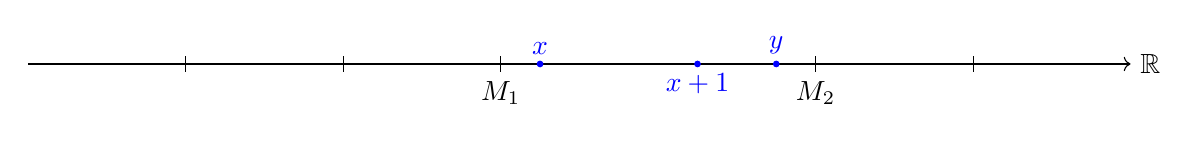
\begin{tikzpicture}[x=2cm]
  \draw[->] (-1,0) -- (6,0) node[right] {$\mathbb{R}$};

  \foreach \x in {0,1,2,4,5}
    \draw (\x,0.1) -- (\x,-0.1);

  \draw (2, 0.1) -- (2, -0.1) node[below] {$M_1$};
  \draw (4, 0.1) -- (4, -0.1) node[below] {$M_2$};

  \filldraw[blue] (2.25,0) circle (1pt) node[above] {$x$};
  \filldraw[blue] (3.25,0) circle (1pt) node[below] {$x + 1$};
  \filldraw[blue] (3.75,0) circle (1pt) node[above] {$y$};
\end{tikzpicture}
\end{center}

What can we say about $M_2 - M_1$? It is clearly more than $1$. Formally, $M_1 < x \iff -x < -M_1$, and we know $x + 1 < M_2$. Adding these inequalities, we get
\begin{align*}
1 < M_2 - M_1\\
\iff 1 + M_1 < M_2
\end{align*}
But $M_1$ and $M_2$ are natural numbers. If $1 + M_1$ is strictly smaller than $M_2$, can I say there is a natural number between $M_1$ and $M_2$? Yes! $1 + M_1$ is such a number
$$
M_1 < 1 + M_1 < M_2
$$
But is it necessary that $1 + M_1$ will fit between $x$ and $y$? If we had $x < M_1$ and $M_2 < y$, we would have no problems. But instead we have the \emph{exact} opposite -- that $M_1 < x$ and $y < M_2$. It is here that we bring the assumption that $x$ and $y$ are not integers.

Suppose $1 + M_1$ was smaller than $x$, but that would contradict that $M_1$ was the maximum element in $S_1$, hence $1 + M_1 \geq x$. Since $x$ is not an integer, we have the strict inequality $1 + M_1 > x$.

How about $y$? Suppose $M_2 > 1 + M_1 > y$. Again this contradicts the minimality of $M_2$ in $S_2$. Hence $1 + M_1 \leq y$ and again $1 + M_1 < y$. Thus $$x < 1 + M_1 < y$$ And $1 + M_1$ is the required natural number.\qed

\begin{center}
\begin{tikzpicture}[x=2.5cm][y=2cm]
  \draw[->] (-1,0) -- (5,0) node[right] {$\mathbb{R}$};

  \foreach \x in {0,1,3,4}
    \draw (\x,0.1) -- (\x,-0.1);

  \draw (1, 0.1) -- (1, -0.1) node[above, yshift=3.5pt] {$M_1$};
  \draw (2, 0.1) -- (2, -0.1) node[above, yshift=3.5pt] {$1 + M_1$};
  \draw (3, 0.1) -- (3, -0.1) node[above, yshift=3.5pt] {$M_2$};

  \draw[red] (1, 0) -- (1.25, 0);
  \draw[red] (2.25, 0) -- (3, 0);

  \filldraw[blue] (1.25,0) circle (1pt) node[below] {$x$};
  \filldraw[blue] (2.25,0) circle (1pt) node[below] {$x + 1$};
  \filldraw[blue] (2.75,0) circle (1pt) node[below] {$y$};
\end{tikzpicture}\\
$1 + M_1$ cannot lie in the regions marked by the red lines
\end{center}
\end{smrg}
\begin{SNP}{\rmk}{The argument can indeed be extended when one or both of $x$ and $y$ are integers, and even further to allow negative $x$ and $y$. So in general whenever $y - x > 1$ there is an integer $m$ such that $x < m < y$.}
\end{SNP}

\begin{smrg}
\pf (Of Theorem 3.) If $x < 0 < y$ then $r = 0$ suffices. Suppose WLG that $0 < x < y$ (the symmetric case being when $x < y < 0$). Indeed, $y - x > 0$. Thus, by Archimedean property, for some $n$ we must have
$$
n(y - x) > 1
\iff ny - nx > 1
$$
By the lemma we just proved, there must be some natural number $m$ such that
$$
nx < m < ny
$$
and therefore
$$
x < \dfrac{m}{n} < y
$$
Thus $\frac{m}{n}$ is a rational number satisfying the required property. When $x < y < 0$ we have $0 < -y < -x$, and we can proceed similarly.\qed
\end{smrg}
Can we use the density of rationals to prove the Archimedean Property? Well, if there is always a rational number $\frac{m}{n}$ such that $x < \frac{m}{n} < x + 1$ for every $x > 0$, then certainly $x \leq nx < m$ and thus $x$ is not an upper bound.
\begin{SNP}{\ex}{Explain why the above ``proof'' of the Archimedean property using the density of rationals is circular. (Hint. How did we guarantee the existence of $M_2$ and $M_1$?)}
\end{SNP}

\AnswerSection
\ans When we are proving the density of $\bb Q$, we use Lemma 1, the proof of which relies on the Archimedean property (to guarantee that some $M_2$ is $> y$ and that $x$ is not an upper bound of $S_1$). So using density to prove Archimedean property already assumes the Archimedean property and is hence circular. 

\end{document}